
\documentclass[11pt,a4paper,openany]{report}
\usepackage[T1]{fontenc}
\usepackage[utf8]{inputenc}
\usepackage{lmodern}
\usepackage{microtype}
\usepackage{amsmath,amssymb,amsthm,mathtools,bm}
\usepackage{booktabs,array,longtable,tabularx}
\usepackage{xcolor}
\usepackage[margin=22mm,headheight=23pt]{geometry}
\usepackage{enumitem}
\usepackage{fancyhdr}
\usepackage{fancyvrb}
\usepackage{graphicx}
\usepackage{url}
\usepackage{xurl}
\usepackage{hyperref}
\definecolor{finblue}{HTML}{1F5A99}
\definecolor{fingreen}{HTML}{19733A}
\definecolor{finorange}{HTML}{D55E00}
\definecolor{finred}{HTML}{A61B1B}
\definecolor{finviolet}{HTML}{6A3D9A}
\definecolor{fingray}{HTML}{4D4D4D}

\hypersetup{
  unicode=true,
  colorlinks=true,
  linkcolor=finblue,
  citecolor=fingreen,
  urlcolor=finblue,
  pdftitle={FIN Research Programs P309--P322},
  pdfauthor={Krzysztof Żuchowski},
  pdfsubject={Bridge-resource lower bounds, operational separation, and sector-role obstruction},
  pdfkeywords={FIN, signed path resource, Hausdorff moment, nontorsion phase, common parent, operational distance, clock identifiability, sector pointing}
}
\pagestyle{fancy}
\fancyhf{}
\fancyhead[L]{\small FIN Programs P309--P322}
\fancyhead[R]{\small Release 10.28}
\fancyfoot[C]{\thepage}

\setlength{\parindent}{0pt}
\setlength{\parskip}{0.55em}
\setlist{nosep,leftmargin=2em}
\setcounter{tocdepth}{2}
\setcounter{secnumdepth}{3}
\emergencystretch=3em
\newcommand{\one}{\bm 1}
\newcommand{\C}{\mathbb C}
\newcommand{\R}{\mathbb R}
\newcommand{\Z}{\mathbb Z}
\newcommand{\statusProven}{\textcolor{fingreen}{[Proven]}}
\newcommand{\statusStrong}{\textcolor{finblue}{[Strong evidence]}}
\newcommand{\statusModerate}{\textcolor{finviolet}{[Moderate evidence]}}
\newcommand{\statusWeak}{\textcolor{fingray}{[Weak evidence]}}
\newcommand{\statusSpeculative}{\textcolor{finorange}{[Speculative]}}
\newcommand{\statusRefuted}{\textcolor{finred}{[Refuted]}}

\begin{document}
\hypersetup{pageanchor=false}
\begin{titlepage}
\centering
\vspace*{7mm}
{\Large\bfseries FIN --- Release 10.28\par}
\vspace{9mm}
{\Huge\bfseries Research Programs P309--P322\par}
\vspace{6mm}
{\Large Bridge-resource lower bounds,\\
operational separation,\\
and the sector-role obstruction\par}
\vspace{13mm}
{\Large Krzysztof \.Zuchowski\par}
\vspace{2mm}
{\normalsize Independent Researcher --- Fractal Information Theory Project\par}
\vspace{2mm}
{\normalsize ORCID:
\href{https://orcid.org/0009-0002-0909-3613}{0009-0002-0909-3613}\par}
\vspace{7mm}
{\large 30 July 2026\par}
{\normalsize Publication --- Preprint; Version 1.0.0\par}
\vfill
\begin{minipage}{0.92\textwidth}
\small
\textbf{Central result.}
Strict attenuation lies outside the positive path-scale cone and requires
signed negative mass at least \(0.0715275581\) in the declared moment
representation.  Its frozen phase tuple additionally requires one
infinite-order generator not contained in the finite legacy phase group.

\medskip
\textbf{Bridge boundary.}
A cross-supported common parent exists after an explicit legacy positivity
repair, but it imports the strict operator.  The remaining bridge-resource
budget keeps signed path weight, nontorsion phase, cross law, pointing, scale,
and operational records separately typed.

\medskip
\textbf{Repository.}
\url{https://github.com/hyconiek/Fractal-Nadsoliton-Theory}

\textbf{License.} CC BY 4.0.
\end{minipage}
\vfill
\end{titlepage}
\hypersetup{pageanchor=true}
\pagenumbering{roman}
\chapter*{Publication statement}
\addcontentsline{toc}{chapter}{Publication statement}
This monograph reports all executed Programs P309--P322 and recommends
Programs P323--P336. Mathematical proof, target-dependent construction,
synthetic evidence, scoped refutation, and missing external evidence remain
separate. The legacy/strict split, QW-2191, dimensional-source, physical-role,
laboratory, \(L_{\rm total}\), and Theory-of-Everything boundaries are
preserved.

\tableofcontents
\clearpage
\pagenumbering{arabic}

\chapter*{Confidence convention}
\addcontentsline{toc}{chapter}{Confidence convention}

\begin{itemize}
\item 
\textbf{\statusProven{}} --- analytic identity, finite theorem, exact arithmetic result, or machine-checked statement in the declared class.

\item 
\textbf{\statusStrong{}} --- reproducible numerical or synthetic audit with frozen inputs, controls, and metrics.

\item 
\textbf{\statusModerate{}} --- stable result depending on an additional equivalence or modeling assumption.

\item 
\textbf{\statusSpeculative{}} --- proposed object without sufficient proof.

\item 
\textbf{\statusRefuted{}} --- counterexample or no-go theorem in the declared class.

\item 
\textbf{[Blocked by external evidence]} --- an executable gate was reached, but independent data, calibration, custody, or hardware were absent.

\end{itemize}

A mathematical construction is not evidence that nature realizes it.

\chapter{Executive summary}

Programs P309--P322 were executed. This round did not search for another pointwise fit between the historical legacy kernel and the strict kernel. Instead, it measured the minimum additional resources demanded by the no-go results of Release 10.27.

The principal result is a quantitative \textbf{Bridge Resource Budget}:

\[
\mathfrak B_{L\to S}
=
(\mathcal N_{\rm path},
r_{\rm phase},
X_{\rm parent},
t_0,
\kappa,
\mathfrak O).
\]

Its components are:

\begin{itemize}
\item 
signed path-scale negativity \(\mathcal N_{\rm path}\);

\item 
an infinite-order phase generator \(r_{\rm phase}\);

\item 
an independently sourced cross-supported parent law \(X_{\rm parent}\);

\item 
operational pointing \(t_0\);

\item 
dimensional scale \(\kappa\);

\item 
operational package \(\mathfrak O\) containing preparations, clock, instrument, environment, and record.

\end{itemize}

The first two components now have rigorous lower-bound or minimal-extension theorems. A cross-supported parent can be constructed, but only by importing both repaired legacy and strict operators. Pointing, scale, and external physical records remain additional.

\section{Signed resource is unavoidable}

For the strict attenuation samples

\[
h_d=\frac{1}{1+d^{1.8}},
\qquad d=0,\ldots,6,
\]

the fourth forward difference is

\[
\Delta^4h_0=-0.07152755810446826.
\]

Every positive exponential-distance mixture is a Hausdorff moment sequence and satisfies

\[
\Delta^4h_0\ge0.
\]

Consequently, every normalized signed representation has Jordan negative mass

\[
\boxed{
\mathcal N_{\rm path}
\ge
0.07152755810446826
}.
\]

Finite moment-grid linear programs give:

\begin{center}
\begingroup\small
\setlength{\tabcolsep}{2.5pt}
\renewcommand{\arraystretch}{1.16}
\begin{longtable}{@{}p{0.182\textwidth}p{0.290\textwidth}p{0.388\textwidth}@{}}
\toprule
\textbf{Moment grid} & \textbf{Minimum negative mass} & \textbf{Moment residual} \\
\midrule
\endhead
61 & 0.4068556 & \(2.60\times10^{-14}\) \\
121 & 0.4067611 & \(2.22\times10^{-16}\) \\
241 & 0.4067109 & \(5.55\times10^{-17}\) \\
\bottomrule
\end{longtable}
\endgroup
\end{center}

The analytic value \(0.07153\) is a rigorous continuum lower bound. The value near \(0.4067\) is a grid-dependent upper bound and optimum inside each declared finite atom set. \textbf{\statusProven{} /\allowbreak{} \statusStrong{}}

This does not prove a quantum interpretation. It proves that positive classical path-scale mixing is insufficient.

\section{One new infinite-order phase generator is necessary}

The legacy phase subgroup generated by

\[
e^{i\pi/4},\qquad e^{i\pi/6}
\]

is finite of order \(24\).

For the frozen strict decimal tuple,

\[
\omega_S=\frac{743}{4000},
\qquad
\phi_S=\frac{13}{80}=\frac{650}{4000}.
\]

Since \(\gcd(743,650)=1\), one generator

\[
r=e^{i/4000}
\]

is sufficient:

\[
e^{i\omega_S}=r^{743},
\qquad
e^{i\phi_S}=r^{650}.
\]

Because \(\pi\) is transcendental, \(r\) has infinite order. A torsion-preserving map from the finite legacy phase group cannot generate it.

\textbf{Verdict:} one infinite-order phase generator is the minimal algebraic extension for the frozen decimal tuple. It is target-coded and is not an internal FIN source. \textbf{\statusProven{}}

\section{A nontrivial parent exists but is not a derivation}

After the explicit absolute-value positivity repair of legacy, define

\[
\mathcal P
=
\begin{pmatrix}
A_L & A_L^{1/2}A_S^{1/2}\\
A_S^{1/2}A_L^{1/2} & A_S
\end{pmatrix}.
\]

For the commuting circulant operators on \(C_{12}\), \(C_{16}\), and \(C_{24}\), this is a positive cross-supported Gram parent. Its rank is \(n-1\), compared with \(2n-2\) for the direct sum. Both principal compressions are exact.

However, the cross block imports \(A_S^{1/2}\). The construction proves compatibility, not generation. A cubic spectral map trained on \(C_{12}\) has RMSE \(0.1053\) on \(C_{12}\), \(0.1633\) on \(C_{16}\), and \(0.2444\) on \(C_{24}\).

\textbf{Verdict:} common-parent existence \textbf{\statusProven{}}; legacy-to-strict source theorem \textbf{[Refuted for this construction]}.

\section{Legacy and strict are operationally distinguishable}

After optimizing one overall legacy time/\allowbreak{}energy scale, the finite operational menu gives:

\begin{center}
\begingroup\small
\setlength{\tabcolsep}{2.5pt}
\renewcommand{\arraystretch}{1.16}
\begin{longtable}{@{}p{0.152\textwidth}p{0.203\textwidth}p{0.238\textwidth}p{0.267\textwidth}@{}}
\toprule
\textbf{Dynamics} & \textbf{Optimized legacy scale} & \textbf{Operational TV distance} & \textbf{Conservative 95\% shot bound} \\
\midrule
\endhead
heat & 0.09394 & 0.23038 & 140 \\
wave & 0.12995 & 0.42207 & 42 \\
\bottomrule
\end{longtable}
\endgroup
\end{center}

The heat comparison uses the explicit absolute-value legacy positivity repair. The wave comparison uses the historical signed self-adjoint legacy generator.

These are finite-menu lower bounds, not global diamond norms. They nevertheless refute operational equivalence under the declared preparations, times, and vertex measurement. \textbf{\statusProven{}}

\section{The old electroweak role still does not transfer}

The quantity

\[
\sin^2\theta_W=\frac{\alpha_{\rm geo}}{12}
\]

cannot be obtained naturally from an unlabelled strict spectrum. The electroweak expression

\[
\frac{g'^2}{g^2+g'^2}
\]

requires an ordered distinction between two sector roles. Sector swap sends the value \(x\) to \(1-x\). A free two-sector swap has no invariant point, and an unlabelled spectrum supplies no ordering.

Five candidate strict scalar invariants were evaluated on \(C_{12}\), \(C_{16}\), and \(C_{24}\). None supplies the missing ordered sector functor, couplings, renormalization semantics, or carrier-independent benchmark.

\textbf{Verdict:} spectrum-only electroweak role transfer \textbf{\statusRefuted{}}. An axiom-augmented sector theory remains possible but must expose its added pointing and coupling data.

\section{Other principal results}

\begin{enumerate}
\item 
Equal-residue pole collision has Gaussian KL divergence \(O(P\delta^4/\sigma^2)\); finite probe count cannot make the Stieltjes inverse uniformly Lipschitz.

\item 
Six E-optimal probes improve the profiled pole-information condition number from \(6.98\times10^5\) to \(4.92\), but do not remove the minimax collision class.

\item 
Lean 4.28 checks the general completion-square implication, the torsion-preserving obstruction, the Boolean sector-swap no-point theorem, and role factorization on kernel fibers.

\item 
A loss/\allowbreak{}no-click/\allowbreak{}detector completion of the \(72\)-mode current mesh remains a POVM with response rank five in every tested realization.

\item 
Every positive mixture of legacy hyperbolic scales has a \(d^{-1}\) lower tail and cannot equal the strict \(d^{-1.8}\) envelope.

\item 
A tuned drift-aware synthetic detector filter improves median gradient RMSE by a factor \(1.55\) over its matched static filter.

\item 
All \(6!=720\) Fourier-mode order chambers are full-dimensionally feasible inside the positive radial-weight simplex in the exhaustive LP audit.

\item 
A cubic clock family becomes locally identifiable only after calibrating \(\tau'(0)=1\); without this reference, four scale/\allowbreak{}clock parameters have rank three.

\item 
No independent P241 laboratory bundle or certified hardware reservoir package was admitted.

\end{enumerate}

No result closes QW-2191, derives the phase generator, derives signed negativity dynamically, sources a dimensional unit, transfers a legacy physical role, validates FIN in a laboratory, promotes \(L_{\rm total}\), or establishes Standard Model, gravitational, or Theory-of-Everything closure.

\begin{figure}[htbp]
\centering
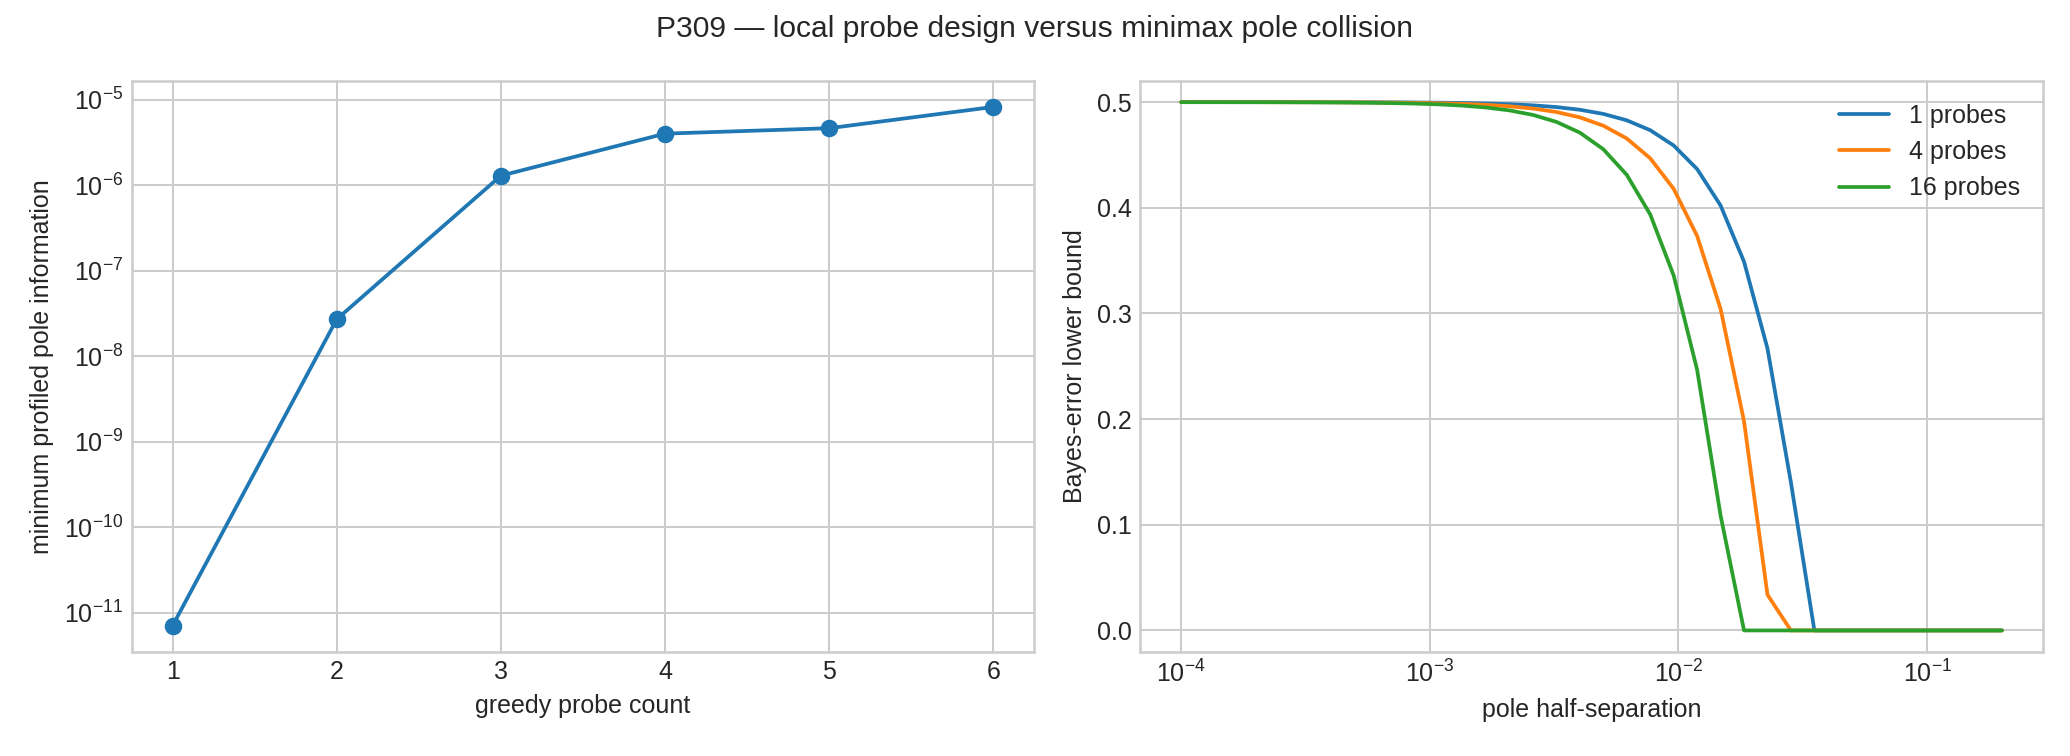
\includegraphics[width=0.97\textwidth]{FIN_Programs_309_322_Figures/p309_minimax_stieltjes.png}
\caption{Finite-probe information improvement and the pole-collision minimax obstruction.}
\end{figure}

\chapter{Scope and retained kernel discipline}

The historical/\allowbreak{}intermediate legacy kernel remains

\[
K_L(d)
=
\alpha_{\rm geo}
\frac{\cos(\pi d/4+\pi/6)}
{1+\beta_{\rm tors}d},
\qquad
\alpha_{\rm geo}=4\ln2,
\quad
\beta_{\rm tors}=0.01.
\]

The strict working kernel remains

\[
K_S(d)
=
\frac{\cos(0.18575d+0.16250)}
{1+d^{1.8}}.
\]

The legacy kernel is an intermediate bridge object and the strict kernel is the later enriched working kernel where explicit completion evidence licenses that description. They are not silently identical.

Three legacy versions are distinguished in this release:

\begin{center}
\begingroup\small
\setlength{\tabcolsep}{2.5pt}
\renewcommand{\arraystretch}{1.16}
\begin{longtable}{@{}p{0.171\textwidth}p{0.349\textwidth}p{0.340\textwidth}@{}}
\toprule
\textbf{Symbol} & \textbf{Meaning} & \textbf{Admissible use} \\
\midrule
\endhead
\(K_L\) & historical signed legacy kernel & wave/\allowbreak{}self-adjoint comparison \\
\(K_{L,\lvert\cdot\rvert}\) & absolute-value positivity repair & explicitly repaired heat/\allowbreak{}parent comparison \\
\(K_S\) & strict working kernel & current positive generator \\
\bottomrule
\end{longtable}
\endgroup
\end{center}

The absolute-value operation is not historical physics and is not a completed bridge. Every result using it says so explicitly.

The ontology remains

\[
\text{nadsoliton}
\to
\text{light}
\to
\text{matter}
\to
\text{emergent observer},
\]

with the nadsoliton treated internally as primordial information in a solitonic state and no lower information layer.

\chapter{The Bridge Resource Budget}

Release 10.27 constructed the Typed Legacy--Strict Completion Span

\[
K_L\leftarrow\mathcal P\rightarrow K_S.
\]

The present round refines the missing data into

\[
\mathfrak B_{L\to S}
=
(\mathcal N_{\rm path},
r_{\rm phase},
X_{\rm parent},
t_0,
\kappa,
\mathfrak O).
\]

\section{Necessity ranking}

\begin{center}
\begingroup\small
\setlength{\tabcolsep}{2.5pt}
\renewcommand{\arraystretch}{1.16}
\begin{longtable}{@{}p{0.221\textwidth}p{0.214\textwidth}p{0.242\textwidth}p{0.183\textwidth}@{}}
\toprule
\textbf{Resource} & \textbf{Present result} & \textbf{Necessity} & \textbf{Current source} \\
\midrule
\endhead
signed path resource \(\mathcal N_{\rm path}\) & lower bound \(0.0715276\) & proven in moment-mixture class & absent \\
infinite-order phase \(r_{\rm phase}\) & one generator \(e^{i/4000}\) & proven for exact frozen tuple & target-coded only \\
parent cross-law \(X_{\rm parent}\) & compatible Gram parent exists & cross support necessary for nontrivial parent & imports strict \\
pointing \(t_0\) & sector swap has no invariant point & proven & absent \\
scale \(\kappa\) & clock/\allowbreak{}scale rank defect & proven & external calibration only \\
operational package \(\mathfrak O\) & finite measurement model constructed & necessary for predictions & synthetic/\allowbreak{}conditional \\
\bottomrule
\end{longtable}
\endgroup
\end{center}

The table is not a claim that these resources are independent in every future theory. It states that the current artifacts do not derive identifications between them.

\section{Removal tests}

\begin{itemize}
\item 
Remove \(\mathcal N_{\rm path}\): strict violates a Hausdorff moment inequality.

\item 
Remove \(r_{\rm phase}\): a finite torsion group cannot reach the strict phase subgroup.

\item 
Remove cross support: the parent degenerates to a direct sum and predicts no relation.

\item 
Remove pointing: sector exchange prevents an ordered physical-role map.

\item 
Remove \(\kappa\): generator scale and clock conversion lie on the same orbit.

\item 
Remove \(\mathfrak O\): there is no outcome law and therefore no experiment.

\end{itemize}

The smallest honest bridge is consequently not a single scalar renormalization.

\chapter{New objects O62--O73}

\section{O62 --- Minimax Spectral Resolution Modulus}

For a probe class \(\mathcal C\), noise \(\sigma\), and testing error \(\varepsilon\), define

\[
\delta_{\rm res}(\sigma,\mathcal C,\varepsilon)
\]

as the largest pole half-separation that remains indistinguishable in a declared worst-case subfamily.

For equal residues,

\[
\delta_{\rm res}
=
O\left(
\sigma^{1/2}P^{-1/4}
\right).
\]

\textbf{Status:} worst-case scaling \textbf{\statusProven{}}.

\section{O63 --- Loss-Completed Measurement Package}

\[
\mathfrak M_{\rm loss}
=
(U,\mathbf T,E_{\varnothing},C_{\rm det},
\mathcal K_{\rm cal}).
\]

Here \(U\) is the unitary mesh, \(\mathbf T\) mode transmissions, \(E_{\varnothing}\) the no-click effect, \(C_{\rm det}\) the detector confusion channel, and \(\mathcal K_{\rm cal}\) calibration data.

\textbf{Status:} algebraically constructed; calibration is synthetic.

\section{O64 --- Joint Feature Parent}

\[
\mathcal P_{\rm JF}
=
\begin{pmatrix}
A_L & X\\
X^\ast & A_S
\end{pmatrix},
\qquad
X=A_L^{1/2}A_S^{1/2}.
\]

It is nontrivial because \(X\ne0\) and its rank is lower than the direct-sum rank.

\textbf{Status:} \textbf{[Constructed]} after positivity repair; not source independent.

\section{O65 --- Regular-Variation Bridge Class}

For path count \(N(d)\sim d^p\) and weight \(w(d)\sim d^{-q}\), define bridge index

\[
\rho=p-q.
\]

The historical stated pair gives \(\rho=1\); legacy requires \(\rho=-1\); strict attenuation requires \(\rho=-1.8\).

\textbf{Status:} \textbf{[Defined]}; the historical counting explanation is refuted.

\section{O66 --- Minimal Nontorsion Phase Extension}

\[
\mathcal R_\phi
=
\langle r\rangle,
\qquad
r=e^{i/4000}.
\]

It is the smallest cyclic infinite-order extension generating both frozen strict phase parameters in integer powers.

\textbf{Status:} \textbf{[Proven minimal]} for exact frozen decimals; not sourced.

\section{O67 --- Operational Kernel Pseudometric}

\[
d_{\mathcal C}(A,B)
=
\sup_{c\in\mathcal C}
\frac12\|p_A^c-p_B^c\|_1.
\]

P315 evaluates it on a finite vertex/\allowbreak{}time menu after optimizing the legacy scale.

\textbf{Status:} finite-menu lower bounds \textbf{\statusProven{}}.

\section{O68 --- Signed Path Resource}

For a signed measure

\[
\nu=\nu_+-\nu_-,
\]

define

\[
\mathcal N(\nu)=\nu_-(\Omega).
\]

It measures departure from the positive path-mixture cone.

\textbf{Status:} strict lower bound \textbf{\statusProven{}} in the moment representation.

\section{O69 --- Drift-Aware Sequential Instrument}

\[
\mathfrak I_{\rm drift}
=
(\mathcal L_{\rm det},Q_{\rm drift},
\mathcal S_{\rm cal},\Pi_{\rm stop}).
\]

The entries are detector likelihood, process prior, calibration cadence, and posterior stop/\allowbreak{}coverage rule.

\textbf{Status:} synthetic construction \textbf{\statusStrong{}}.

\section{O70 --- Spectral Chamber Complex}

The positive radial simplex is stratified by the ordering of six nonzero Fourier-mode values. Its maximal open cells are spectral order chambers.

\textbf{Status:} at most \(720\) chambers \textbf{\statusProven{}}; all \(720\) feasible and rank five at LP centers \textbf{\statusStrong{}}.

\section{O71 --- Clock Identifiability Certificate}

\[
\mathsf{ClockID}
=
(\mathcal T_{\rm family},
\tau'(0),
\mathcal D,
I_{\mathcal D}).
\]

It contains a restricted clock family, reference slope, experimental design, and full-rank Fisher information.

\textbf{Status:} constructed for the cubic clock family. It does not define a canonical clock.

\section{O72 --- Two-Sector Pointing Obstruction}

The ordered pair of sector roles is a free \(\mathbb Z_2\)-torsor. An unlabelled operator does not choose a point of it.

\textbf{Status:} \textbf{\statusProven{}}.

\section{O73 --- Minimal Bridge Resource Budget}

\[
\mathfrak B_{L\to S}
=
(\mathcal N_{\rm path},
\mathcal R_\phi,
\mathcal P_{\rm JF},
t_0,
\kappa,
\mathfrak O).
\]

This higher-generation object assembles the separate no-go boundaries without claiming that they are internally generated.

\textbf{Status:} \textbf{[Constructed as a typed obligation object]}.

\begin{figure}[htbp]
\centering
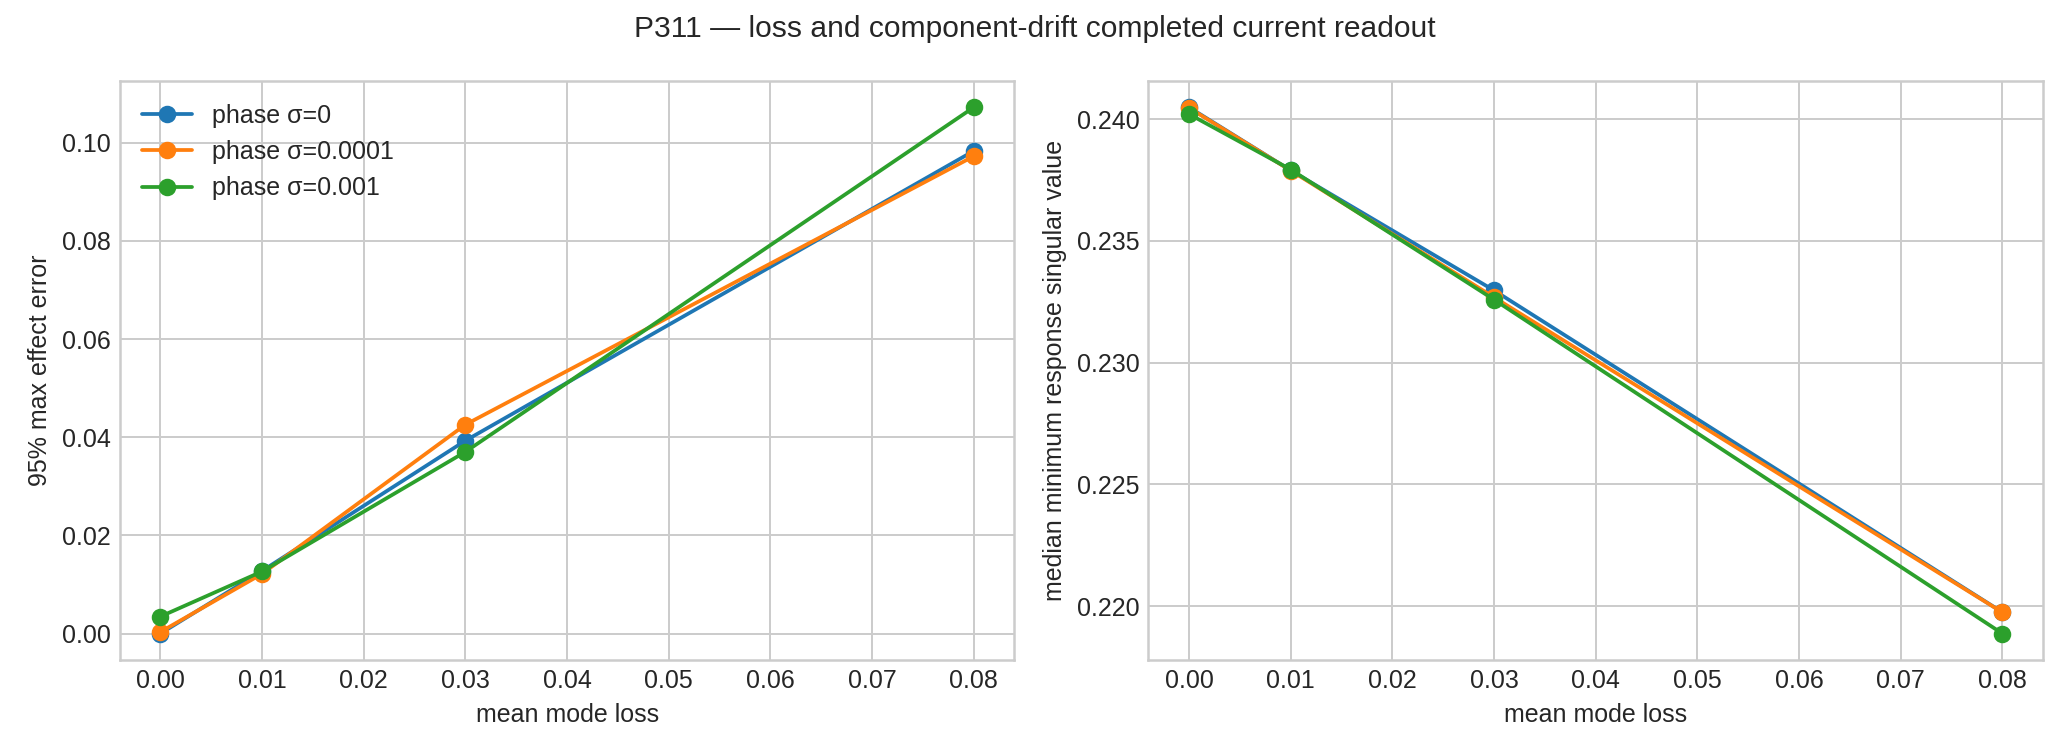
\includegraphics[width=0.97\textwidth]{FIN_Programs_309_322_Figures/p311_lossy_mesh.png}
\caption{Loss, phase drift, no-click completion, and detector response of the synthetic current readout.}
\end{figure}

\chapter{Program results P309--P322}

\section{P309 --- Minimax multi-probe Stieltjes theorem}

For an equal-residue pole pair \(\mu\pm\delta\),

\[
\frac{w}{z+\mu-\delta}
+\frac{w}{z+\mu+\delta}
=
\frac{2w}{z+\mu}
+\frac{2w\delta^2}{(z+\mu)^3}
+O(\delta^4).
\]

Thus the mean response differs from the merged pole only at order \(\delta^2\). With \(P\) independent probes and relative Gaussian noise \(\sigma\),

\[
D_{\rm KL}
=
O\left(
\frac{P\delta^4}{\sigma^2}
\right).
\]

Pinsker and Le Cam give a nonzero testing-error lower bound at

\[
\delta=O(\sigma^{1/2}P^{-1/4}).
\]

The numerical KL exponent is \(4.000008\).

A greedy E-optimal design for the frozen strict atoms gives:

\begin{center}
\begingroup\small
\setlength{\tabcolsep}{2.5pt}
\renewcommand{\arraystretch}{1.16}
\begin{longtable}{@{}p{0.147\textwidth}p{0.405\textwidth}p{0.308\textwidth}@{}}
\toprule
\textbf{Probes} & \textbf{Minimum profiled pole information} & \textbf{Condition number} \\
\midrule
\endhead
1 & \(7.08\times10^{-12}\) & \(6.98\times10^5\) \\
3 & \(1.29\times10^{-6}\) & 23.77 \\
6 & \(8.24\times10^{-6}\) & 4.92 \\
\bottomrule
\end{longtable}
\endgroup
\end{center}

\textbf{Verdict:} finite probes improve local conditioning but cannot remove the worst-case collision modulus. \textbf{\statusProven{} /\allowbreak{} \statusStrong{}}

\section{P310 --- General Schur completion logic}

For

\[
Q(x,y)
=
x^\ast A x
+2\operatorname{Re}x^\ast By
+y^\ast Cy,
\qquad C\succ0,
\]

the completion identity is

\[
Q(x,y)
=
x^\ast(A-BC^{-1}B^\ast)x
+(y+C^{-1}B^\ast x)^\ast
C(y+C^{-1}B^\ast x).
\]

Lean proves abstractly that an exact decomposition into a reduced value plus a nonnegative remainder makes the zero-remainder point a global inner minimizer. Three hundred exact rational block constructions satisfy the full matrix identity.

The repository environment does not contain Mathlib, so a primitive finite-matrix formalization from positive-definiteness assumptions was not completed.

\textbf{Verdict:} mathematical theorem and abstract formal implication \textbf{\statusProven{}}; full Mathlib implementation \textbf{[Blocked by dependency]}.

\section{P311 --- Loss-completed current readout}

The ideal \(72\)-mode unitary is perturbed at its 1,428 complex Givens components. Per-mode loss, detector efficiency, crosstalk, dark counts, and a no-click outcome are then applied.

Across \(144\) realizations:

\begin{itemize}
\item 
every response rank is five;

\item 
maximum POVM completeness residual is \(4.45\times10^{-16}\);

\item 
the minimum observed effect eigenvalue is positive;

\item 
at mean loss \(0.08\) and phase error \(10^{-3}\), the 95th percentile maximum effect error is \(0.1072\);

\item 
the median minimum response singular value decreases from \(0.2405\) to \(0.2189\).

\end{itemize}

\textbf{Verdict:} loss-completed POVM algebra \textbf{\statusProven{}}; tolerance audit \textbf{[Strong evidence, synthetic]}.

\section{P312 --- Cross-supported common parent}

\begin{center}
\begingroup\fontsize{7}{8.4}\selectfont
\setlength{\tabcolsep}{2.5pt}
\renewcommand{\arraystretch}{1.16}
\begin{longtable}{@{}p{0.124\textwidth}p{0.118\textwidth}p{0.189\textwidth}p{0.209\textwidth}p{0.220\textwidth}@{}}
\toprule
\textbf{Carrier} & \textbf{Parent rank} & \textbf{Direct-sum rank} & \textbf{Normalized cross support} & \textbf{C12-trained cubic RMSE} \\
\midrule
\endhead
12 & 11 & 22 & 0.9629 & 0.1053 \\
16 & 15 & 30 & 0.9604 & 0.1633 \\
24 & 23 & 46 & 0.9568 & 0.2444 \\
\bottomrule
\end{longtable}
\endgroup
\end{center}

The historical signed legacy generators have negative eigenvalues \(-21.38\), \(-18.67\), and \(-33.33\), so the parent uses the explicitly repaired absolute-value legacy Laplacians.

\textbf{Verdict:} a shared feature geometry exists, but its cross law imports strict and does not explain strict. \textbf{[Proven construction] /\allowbreak{} [Refuted source claim]}

\section{P313 --- Mellin and regular-variation obstruction}

Every nonzero positive measure on \(\beta>0\) produces

\[
h(d)
=
\int\frac{d\mu(\beta)}{1+\beta d}
\not=o(d^{-1}).
\]

Indeed, some compact interval \([a,b]\) has positive mass, giving

\[
h(d)\ge\frac{\mu([a,b])}{1+bd}.
\]

Strict has

\[
h_S(d)\sim d^{-1.8}=o(d^{-1}),
\]

so no positive mixture of legacy hyperbolic scales can equal it globally.

A nonnegative least-squares fit on \(d=1,\ldots,6\) already has relative residual \(0.1491\). Its extrapolated slope is \(-1.0000\), versus strict \(-1.8000\).

\textbf{Verdict:} \textbf{[Proven scoped no-go]}.

\begin{figure}[htbp]
\centering
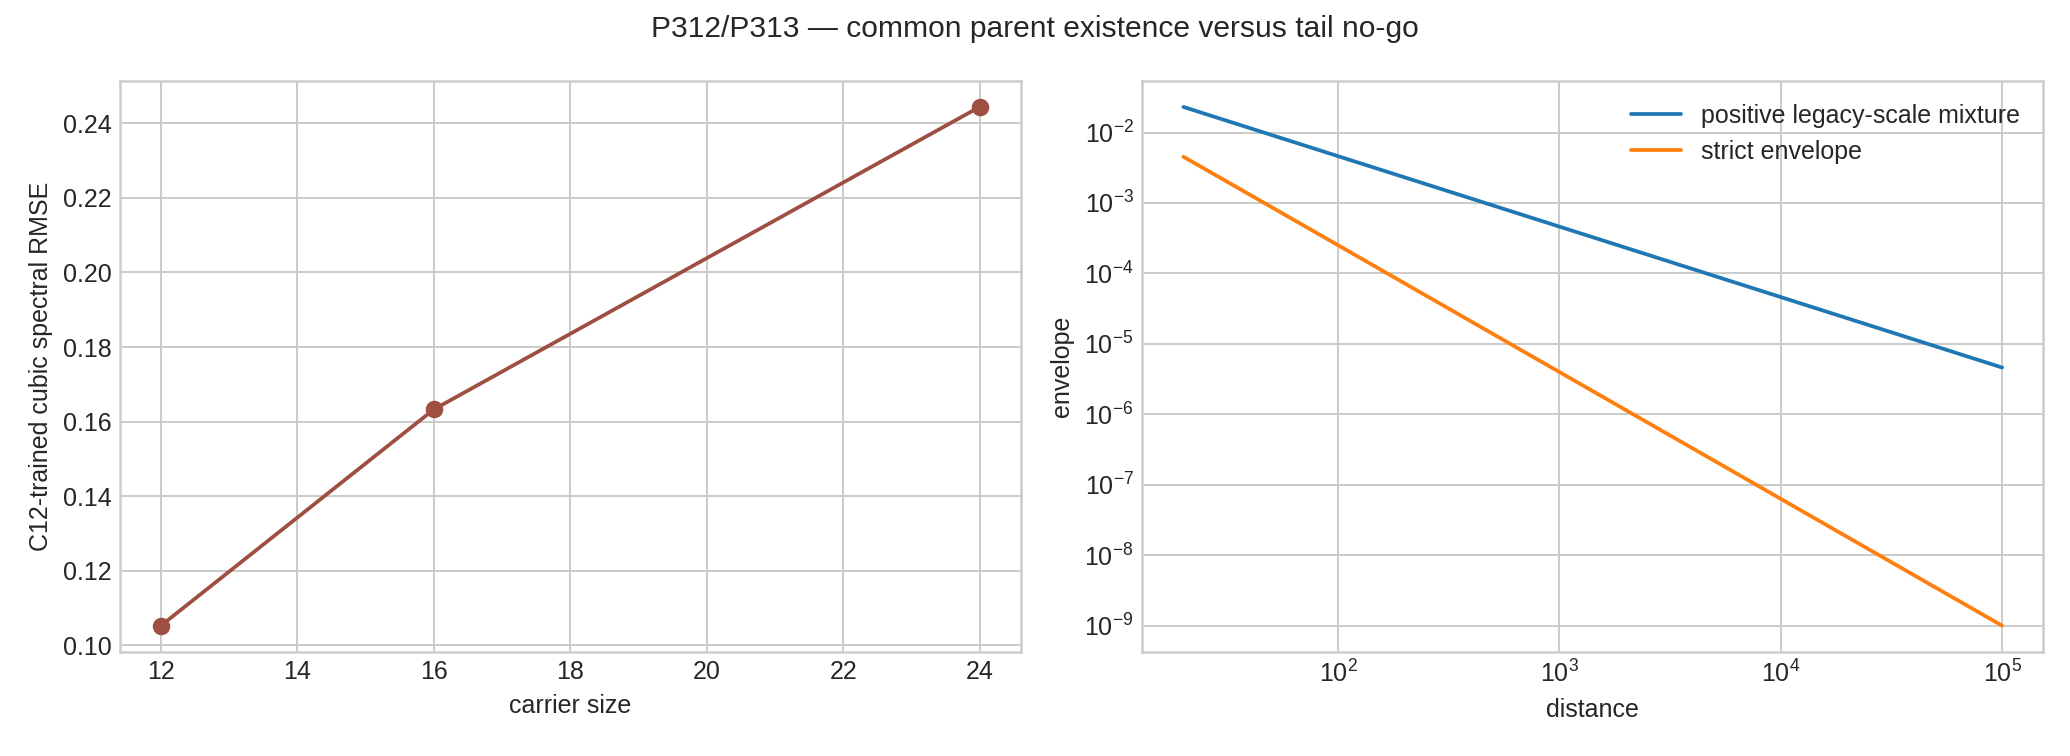
\includegraphics[width=0.97\textwidth]{FIN_Programs_309_322_Figures/p312_p313_parent_tail.png}
\caption{A target-dependent joint-feature parent and the positive hyperbolic-mixture tail obstruction.}
\end{figure}

\section{P314 --- Torsion-to-nontorsion phase theorem}

The exact frozen strict decimals generate the infinite cyclic phase subgroup

\[
\langle e^{i/4000}\rangle.
\]

Lean verifies the abstract theorem that a torsion-preserving map misses a declared nontorsion target.

\textbf{Verdict:} the finite legacy phase group cannot source the strict phase. One infinite-order phase extension is minimal, but supplied. \textbf{\statusProven{}}

\section{P315 --- Operational prediction distance}

The finite menu contains all twelve vertex preparations, vertex measurement, and 42 times between \(0.02\) and \(3\).

The heat witness occurs at \(t=0.78215\), preparation vertex \(7\), with event probabilities:

\[
p_S=0.76503,
\qquad
p_L=0.53466.
\]

The wave witness occurs at \(t=1.62834\), preparation vertex \(2\):

\[
p_S=0.62026,
\qquad
p_L=0.19819.
\]

\textbf{Verdict:} finite-menu operational equivalence is refuted even after optimizing the legacy scale. \textbf{\statusProven{}}

\section{P316 --- Minimum signed path resource}

The fourth-difference theorem gives the continuum lower bound

\[
\mathcal N_{\rm path}\ge0.0715275581.
\]

The grid sequence \(0.406856\), \(0.406761\), \(0.406711\) is stable under doubling the moment-node resolution. The finest representation uses six positive and one negative active atoms.

\textbf{Verdict:} a nonzero signed resource is unavoidable in this path-scale representation. Its dynamical origin is unknown. \textbf{\statusProven{} /\allowbreak{} [Strong evidence]}

\begin{figure}[htbp]
\centering
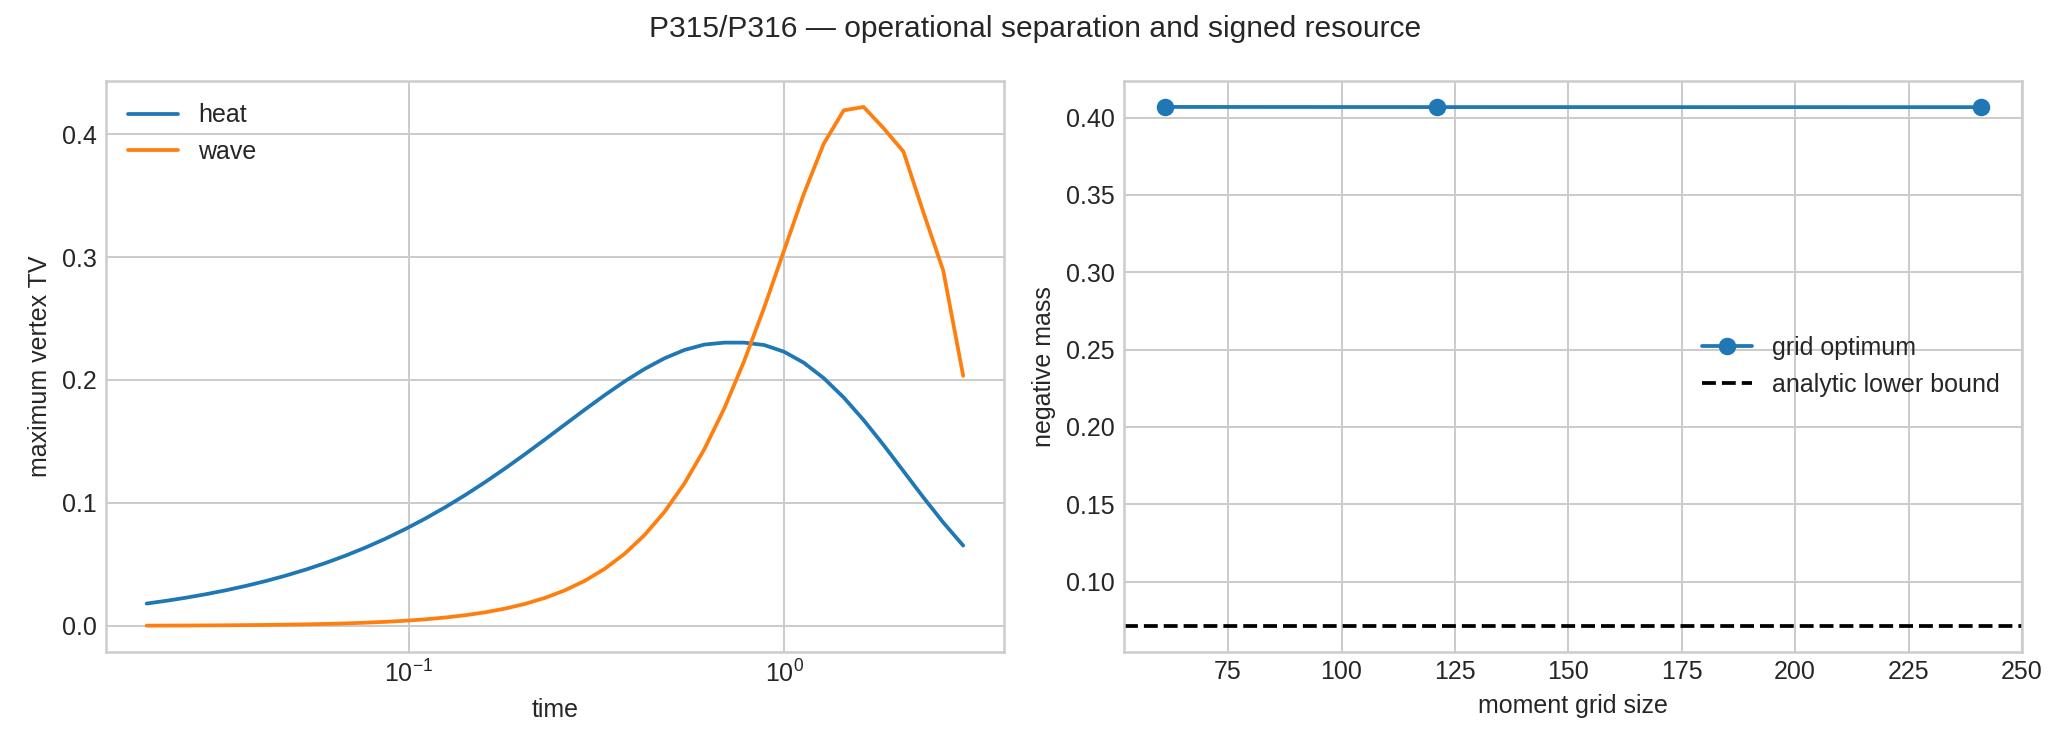
\includegraphics[width=0.97\textwidth]{FIN_Programs_309_322_Figures/p315_p316_distance_negativity.png}
\caption{Operational legacy/strict separation and signed path-resource bounds.}
\end{figure}

\section{P317 --- Independent laboratory intake}

No non-template manifest contains the complete provider, registrar, analyst, hold-out hash, event-file hash, and custody fields required by the P241 gate.

\textbf{Verdict:} \textbf{[Blocked by external evidence]}. P242 remains unauthorized.

\section{P318 --- Sequential detector drift}

The synthetic detector parameters follow a supplied random walk. A Laplace/\allowbreak{}extended-Kalman update uses physics observations and periodic dark, crosstalk, and contrast calibration blocks.

For calibration every block:

\begin{center}
\begingroup\small
\setlength{\tabcolsep}{2.5pt}
\renewcommand{\arraystretch}{1.16}
\begin{longtable}{@{}p{0.314\textwidth}p{0.273\textwidth}p{0.273\textwidth}@{}}
\toprule
\textbf{Filter} & \textbf{Median gradient RMSE} & \textbf{Median 95\% coverage} \\
\midrule
\endhead
static & 0.007667 & 0.642 \\
drift-aware & 0.004954 & 1.000 \\
\bottomrule
\end{longtable}
\endgroup
\end{center}

The RMSE improvement factor is \(1.55\). Dynamic filtering is not uniformly better for every tested cadence, confirming that process-noise tuning and calibration scheduling are part of the model.

\textbf{Verdict:} \textbf{[Strong evidence, synthetic]}.

\section{P319 --- Spectral chamber complex}

Six nonzero Fourier-mode values admit at most

\[
6!=720
\]

strict orders. An exhaustive linear program finds all \(720\) chambers full-dimensionally feasible in the positive radial simplex. Every chamber center has fingerprint Jacobian rank five.

This means mode ordering alone is maximally nonselective. The rarity of the strict fingerprint, when present under a declared null, lies in metric coordinates inside a chamber and not in the mere existence of its order.

For the P289 single-target probability \(2.9\times10^{-8}\), the formal Bonferroni upper bounds are:

\begin{center}
\begingroup\small
\setlength{\tabcolsep}{2.5pt}
\renewcommand{\arraystretch}{1.16}
\begin{longtable}{@{}p{0.420\textwidth}p{0.420\textwidth}@{}}
\toprule
\textbf{Target count} & \textbf{Upper bound} \\
\midrule
\endhead
1 & \(2.9\times10^{-8}\) \\
10 & \(2.9\times10^{-7}\) \\
100 & \(2.9\times10^{-6}\) \\
720 & \(2.088\times10^{-5}\) \\
\bottomrule
\end{longtable}
\endgroup
\end{center}

These numbers apply only if the individual targets share the declared P289 null and bound.

\textbf{Verdict:} finite chamber count and union rule \textbf{\statusProven{}}; exhaustive feasibility/\allowbreak{}rank \textbf{\statusStrong{}}.

\begin{figure}[htbp]
\centering
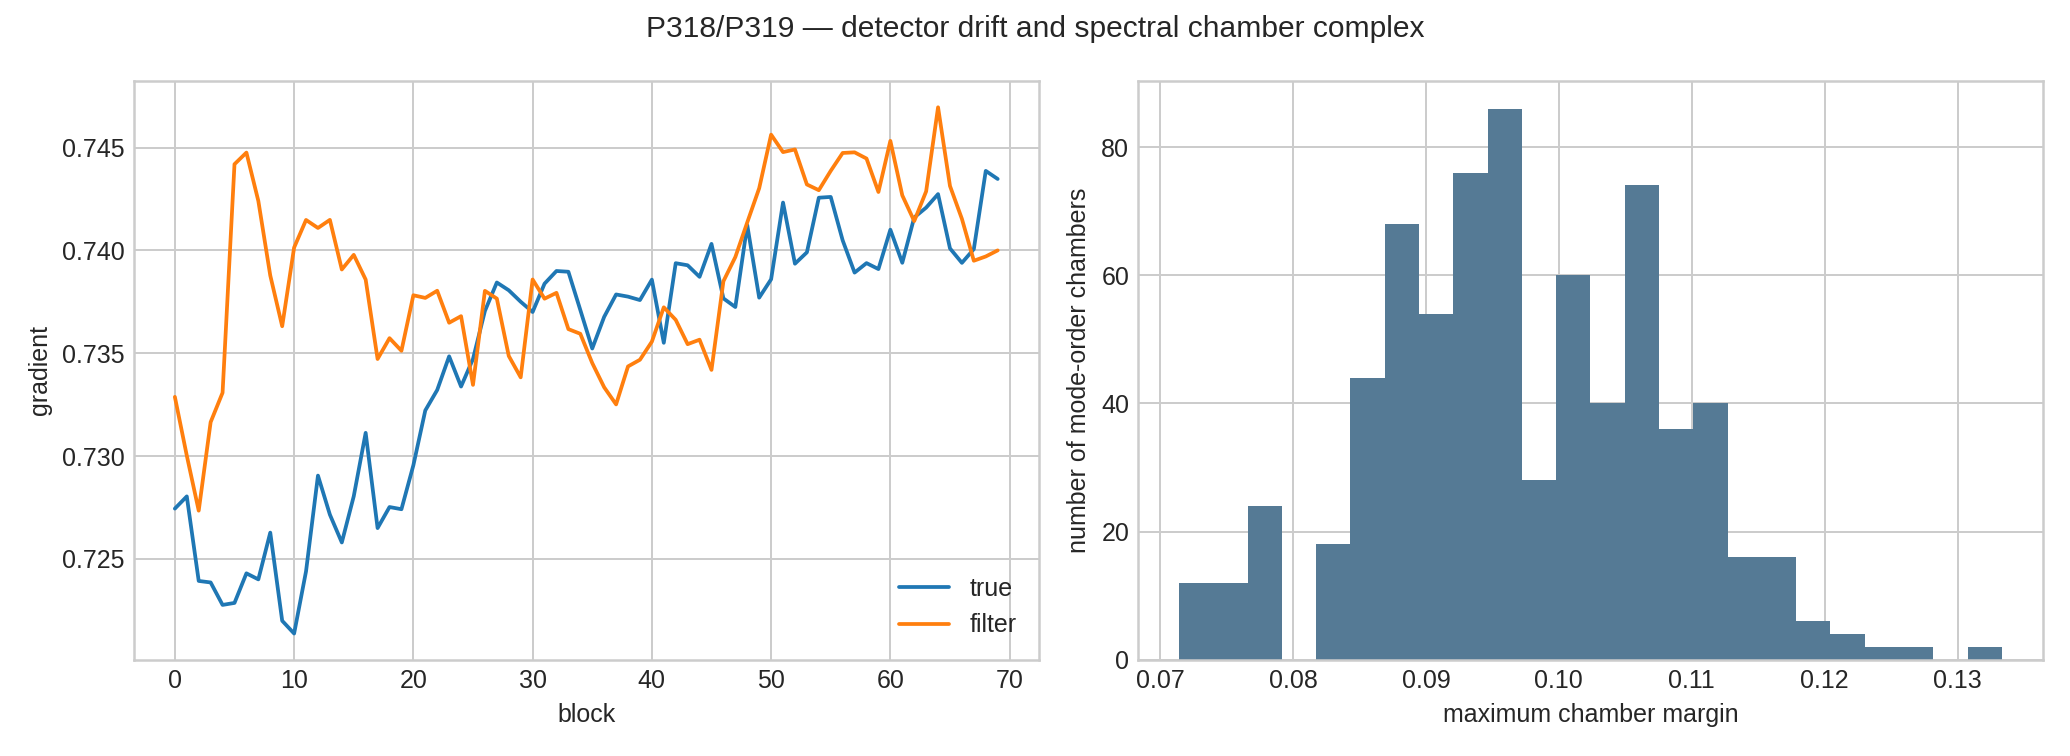
\includegraphics[width=0.97\textwidth]{FIN_Programs_309_322_Figures/p318_p319_drift_chambers.png}
\caption{Synthetic detector drift tracking and the spectral chamber complex.}
\end{figure}

\section{P320 --- Restricted-clock experiment}

The restricted family is

\[
\tau(t)=t+bt^2+ct^3,
\]

after externally calibrating

\[
\tau'(0)=1.
\]

Among 495 four-time designs, the E-optimal set is

\[
(0.05,\;0.154545,\;0.677273,\;1.2).
\]

Its minimum Fisher eigenvalue is \(43.59\), compared with \(18.06\) for \((0.15,0.35,0.65,1.0)\), an improvement factor \(2.41\).

Without the slope calibration, generator scale and the three polynomial clock coefficients give four parameters but sensitivity rank three.

\textbf{Verdict:} restricted local clock identification \textbf{\statusStrong{}}; scale/\allowbreak{}clock rank obstruction \textbf{\statusProven{}}.

\section{P321 --- Physical reservoir gate}

No admitted package contains hardware events, calibrated clock and detector records, paired controls, and a frozen primary endpoint.

\textbf{Verdict:} \textbf{[Blocked by external evidence]}.

\section{P322 --- Electroweak role naturality}

Five candidate scalar invariants were evaluated:

\begin{itemize}
\item 
normalized spectral gap;

\item 
trace-square ratio;

\item 
normalized spectral entropy;

\item 
zero-mode fraction;

\item 
\(\alpha_{\rm geo}/n\).

\end{itemize}

None supplies the required ordered \(U(1)\)/\allowbreak{}\(SU(2)\) sector functor or coupling observables. Their carrier ranges are nonzero; even the most stable spectral entropy is numerically unrelated to the legacy benchmark.

Lean proves:

\begin{enumerate}
\item 
Boolean sector swap has no invariant point;

\item 
every role factoring through a kernel is constant on that kernel's fibers.

\end{enumerate}

The certificate fails all six requirements:

\begin{itemize}
\item 
typed completion naturality;

\item 
ordered sector functor;

\item 
strict \(g',g\) observables;

\item 
renormalization-scale semantics;

\item 
carrier/\allowbreak{}representation invariance;

\item 
independent experimental hold-out.

\end{itemize}

\textbf{Verdict:} current electroweak role transfer \textbf{\statusRefuted{}}.

\begin{figure}[htbp]
\centering
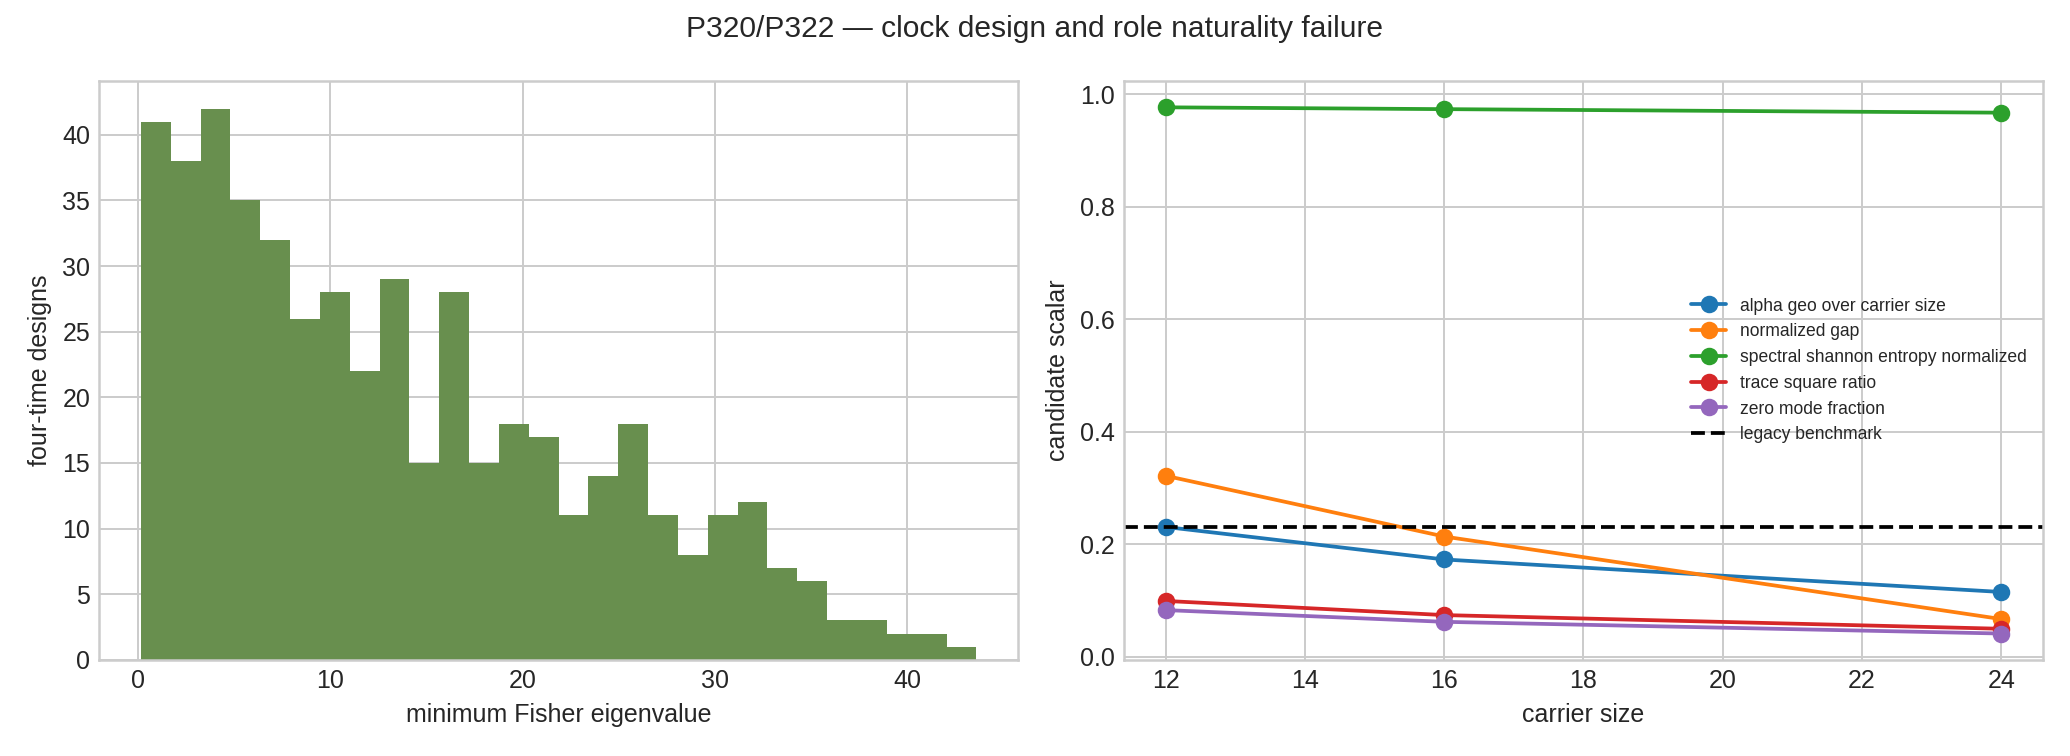
\includegraphics[width=0.97\textwidth]{FIN_Programs_309_322_Figures/p320_p322_clock_role.png}
\caption{Restricted-clock design and carrier dependence of candidate physical role scalars.}
\end{figure}

\chapter{Cross-program synthesis}

\section{What is now known about the bridge}

The following candidate statement is false:

\[
\text{strict}
=
\text{positive rescaling/mixture of legacy}.
\]

It fails independently at four levels:

\begin{enumerate}
\item 
sign and moment-cone inequalities;

\item 
regular-variation tail;

\item 
torsion versus nontorsion phase;

\item 
operational outcome laws.

\end{enumerate}

The smallest surviving bridge class is:

\[
\boxed{\begin{gathered}
\text{signed/noncommutative completion}
+\text{new phase resource}
+\text{independent cross-law}\\
+\text{operational and dimensional references}
\end{gathered}}.
\]

This is a necessity statement, not a constructed physical theory.

\section{Why the common parent is useful despite not being a derivation}

The Joint Feature Parent demonstrates that repaired legacy and strict can be represented as two compressions of one lower-rank feature geometry. It therefore provides:

\begin{itemize}
\item 
a common Hilbert-space test bed;

\item 
a place to define cross-observables;

\item 
a candidate dilation for operational comparison;

\item 
a precise source-independence test.

\end{itemize}

Its failure is equally informative: if a parent cross block uses \(A_S^{1/2}\), it explains nothing about why strict exists. P324 should demand that the cross law be computed from legacy plus independently declared resources before strict is revealed.

\section{Information versus physics}

Signed path weight is not automatically quantum amplitude. An infinite-order phase is not automatically physical time. A unitary mesh is not automatically an apparatus. A sector torsor is not automatically electroweak gauge theory.

The correct chain remains

\[
\text{mathematical resource}
\to
\text{operational implementation}
\to
\text{calibrated event law}
\to
\text{external test}.
\]

The current release advances the first two stages conditionally and does not claim the last two.

\section{Deepest interpretation surviving this round}

FIN remains best interpreted as a finite spectral-information dynamics whose strict generator supports wave, heat, measurement, and information constructions. The historical legacy kernel is a meaningful positive multiscale carrier only after separating its signed phase from its positive envelope.

The strict kernel is not merely a renormalized positive legacy mixture. Its mathematical completion requires at least a signed path resource and an infinite-order phase extension. Physical interpretation additionally requires sector pointing, clock/\allowbreak{}scale calibration, instruments, and records.

\chapter{Failed approaches and no-go boundaries}

\begin{center}
\begingroup\small
\setlength{\tabcolsep}{2.5pt}
\renewcommand{\arraystretch}{1.16}
\begin{longtable}{@{}p{0.356\textwidth}p{0.180\textwidth}p{0.325\textwidth}@{}}
\toprule
\textbf{Candidate} & \textbf{Verdict} & \textbf{Boundary} \\
\midrule
\endhead
finite probes give uniform spectral inverse & \statusRefuted{} & equal-residue collision has quartic KL \\
positive legacy hyperbola mixture gives strict tail & \statusRefuted{} & cannot decay faster than \(d^{-1}\) \\
positive exponential path measure gives strict moments & \statusRefuted{} & negative fourth difference \\
finite legacy phase group gives strict phase & \statusRefuted{} & torsion cannot generate nontorsion \\
common parent proves generation & \statusRefuted{} & cross block imports strict \\
scale-aligned operational equivalence & \statusRefuted{} & heat/\allowbreak{}wave TV witnesses \\
spectral order selects strict & \statusRefuted{} & all 720 orders feasible \\
uncalibrated clock determines generator scale & \statusRefuted{} & rank \(3<4\) \\
unlabelled spectrum transfers EW role & \statusRefuted{} & free sector swap \\
repository simulations validate physics & [Blocked] & no admitted external bundle \\
\bottomrule
\end{longtable}
\endgroup
\end{center}

\chapter{Recommended Programs P323--P336}

Probabilities estimate the chance of a decisive result, including a rigorous no-go. They are research-planning judgments.

\begin{center}
\begingroup\fontsize{7}{8.4}\selectfont
\setlength{\tabcolsep}{2.5pt}
\renewcommand{\arraystretch}{1.16}
\begin{longtable}{@{}p{0.055\textwidth}p{0.092\textwidth}p{0.275\textwidth}p{0.292\textwidth}p{0.145\textwidth}@{}}
\toprule
\textbf{Rank} & \textbf{Program} & \textbf{Study} & \textbf{Decisive output} & \textbf{Probability} \\
\midrule
\endhead
1 & P323 & continuum signed-moment duality & close the gap between \(0.07153\) and \(0.4067\) with an exact dual extremizer & 0.86 \\
2 & P325 & internal phase-source audit & derive or obstruct \(e^{i/4000}\) from target-independent strict information data & 0.84 \\
3 & P324 & source-independent common-parent theorem & classify cross laws computable before access to \(A_S\) & 0.82 \\
4 & P326 & lossy operational discrimination & combine P311 and P315 into an optimal preparation/\allowbreak{}time/\allowbreak{}detector/\allowbreak{}shot protocol & 0.88 \\
5 & P327 & exact algebraic chamber certificate & prove all 720 chamber witnesses over \(\mathbb Q(\sqrt3)\) & 0.80 \\
6 & P328 & quantum comb/\allowbreak{}diamond distance & replace the finite-menu lower bound by an SDP for multitime instruments & 0.73 \\
7 & P329 & clock-model minimax design & optimize against bounded analytic/\allowbreak{}spline clock misspecification & 0.79 \\
8 & P330 & independent P241 execution & run Validator 241 and Pipeline 242 on a real registered event bundle & 0.28 \\
9 & P331 & photonic transfer specification & component list, calibration inversion, loss budget, and preregistered failure thresholds & 0.76 \\
10 & P332 & signed-resource interpretation audit & compare quasi-probability, interference, Krein-space, and open-system realizations without identifying them & 0.70 \\
11 & P333 & non-cyclic common-parent test & repeat source-independent parent criteria on paths, expanders, and irregular graphs & 0.74 \\
12 & P334 & minimal axiom-augmented EW package & add ordered \(U(1)/SU(2)\) sectors and determine the exact extra parameter count & 0.68 \\
13 & P335 & bridge-resource independence theorem & test whether negativity, phase, pointing, and scale form a product obstruction or share one source & 0.66 \\
14 & P336 & external reservoir execution & preregister and run the physical reservoir comparison with paired controls & 0.25 \\
\bottomrule
\end{longtable}
\endgroup
\end{center}

\section{Recommended immediate sequence}

\[
\boxed{
P323
\to
P325
\to
P324
\to
P326
\to
P327
}
\]

This sequence first sharpens the strongest new lower bound, then tests whether the phase resource can be internal, demands a non-target-coded parent, converts operational separation into an apparatus-aware experiment, and replaces floating-point chamber feasibility with exact algebraic certificates.

P330 and P336 remain external gates and must not be simulated into success.

\chapter{Reproducibility}

\section{Executable artifacts}

\begin{itemize}
\item 
fin\_programs\_309\_322.py --- deterministic research runner;

\item 
test\_fin\_programs\_309\_322.py --- regression and boundary suite;

\item 
FIN\_Programs\_309\_322\_Formal\_Core.lean --- Lean 4.28 source;

\item 
FIN\_Programs\_309\_322\_Results.json --- machine-readable results;

\item 
FIN\_Programs\_309\_322\_Summary.csv --- compact program matrix;

\item 
ten detailed CSV tables;

\item 
six figures in FIN\_Programs\_309\_322\_Figures/\allowbreak{}.

\end{itemize}

The random seed is

\[
20260802.
\]

\section{Verification}

Run python3 -m unittest -v test\_fin\_programs\_309\_322.py with MPLCONFIGDIR=/\allowbreak{}tmp/\allowbreak{}mpl-fin.

Expected result: \textbf{17 tests passed, 0 failed.}

\section{Evidence boundary}

Detector drift, losses, phase errors, and finite-count assumptions are synthetic. Exact theorems are scoped to their stated mathematical classes. P317 and P321 certify non-admission rather than create empirical evidence.

\chapter{Final conclusion}

The legacy-to-strict problem has become more precise.

It is no longer scientifically adequate to ask for one better interpolation between two radial formulas. Positive path mixtures, positive hyperbolic scale mixtures, finite phase transport, scalar spectral transport, and unpointed physical-role transfer now have independent obstructions.

The smallest surviving mathematical completion must carry:

\[
\boxed{
\text{signed path resource}
\times
\text{infinite-order phase}
\times
\text{independently sourced cross law}
}.
\]

The smallest surviving physical completion must additionally carry:

\[
\boxed{
\text{sector point}
\times
\text{clock/scale reference}
\times
\text{preparation/instrument/environment/record}
}.
\]

The repository has not derived these resources from one deeper strict principle. It has, however, converted several previously vague missing ingredients into theorem-level lower bounds and executable acceptance tests. That is the scientifically strongest current result.

\chapter{References}

\begin{enumerate}
\item 
N. I. Akhiezer, \emph{The Classical Moment Problem}, Oliver \& Boyd, 1965.

\item 
C. Berg, J. P. R. Christensen, and P. Ressel, \emph{Harmonic Analysis on Semigroups}, Springer, 1984.

\item 
R. Bhatia, \emph{Positive Definite Matrices}, Princeton University Press, 2007.

\item 
S. Boyd and L. Vandenberghe, \emph{Convex Optimization}, Cambridge University Press, 2004.

\item 
L. Le Cam and G. L. Yang, \emph{Asymptotics in Statistics}, Springer, 2000.

\item 
M. A. Naimark, "Spectral functions of a symmetric operator," \emph{Izvestiya Akademii Nauk SSSR} 4 (1940).

\item 
M. G. Krein and A. A. Nudelman, \emph{The Markov Moment Problem and Extremal Problems}, AMS, 1977.

\item 
M. A. Nielsen and I. L. Chuang, \emph{Quantum Computation and Quantum Information}, Cambridge University Press, 2010.

\item 
M. Pollock et al., "Operational Markov condition for quantum processes," \emph{Physical Review Letters} 120 (2018).

\item 
D. V. Widder, \emph{The Laplace Transform}, Princeton University Press, 1941.

\end{enumerate}


\clearpage
\chapter*{Reproduction certificate}
\addcontentsline{toc}{chapter}{Reproduction certificate}
\begin{Verbatim}[fontsize=\small]
MPLCONFIGDIR=/tmp/mpl-fin \
python3 -m unittest -v test_fin_programs_309_322.py
\end{Verbatim}
Expected result: 17 tests passed, 0 failed.  The suite recompiles the
dependency-free Lean 4.28 source.  Loss, detector drift, calibration, and
finite-count assumptions are synthetic.  P317 and P321 admit no external
laboratory or hardware evidence.

\medskip
\noindent\textbf{Suggested citation:}

\.Zuchowski, K. (2026). \emph{FIN Research Programs P309--P322:
Bridge-Resource Lower Bounds, Operational Separation, and the Sector-Role
Obstruction} (Release 10.28; Version 1.0.0) [Preprint]. Zenodo.

\end{document}
